%% ----------------------------------------------------------------
%% AppendixA.tex Circuit Diagrams
%% ---------------------------------------------------------------- 
\chapter{Range Finding Derivations} \label{Appendix:Range}
\begin{figure}
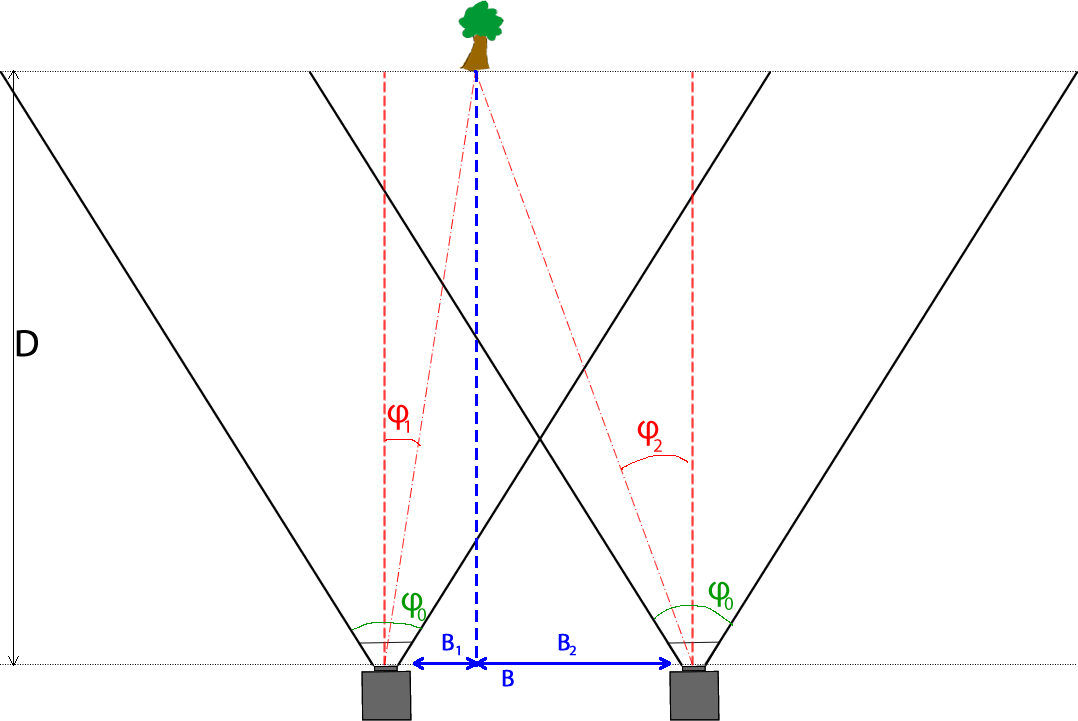
\includegraphics[width=\textwidth,height=\textheight,keepaspectratio]{Figures/problem1.png}
\caption{Problem 1 - Object is between the Cameras}
\label{problem_between}
\end{figure}

\section{Object is between the Cameras}
Derivation from \cite{Mrovlje:Distance_Stereoscopic}.
\begin{equation} \label{eq:B}
B = B_{1} + B_{2} = D\tan(\varphi_{1}) + D\tan(\varphi_{2})
\end{equation}

\begin{equation} \label{eq:D}
D = \frac{B}{\tan(\varphi_{1}) + \tan(\varphi_{2})}
\end{equation}


%\begin{figure}
%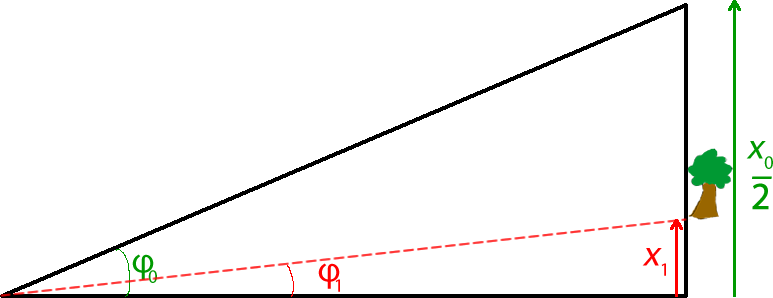
\includegraphics[width=\textwidth,height=\textheight,keepaspectratio]{Figures/left_simplified.png}
%\caption{Problem 1 : Left Camera Simplified}
%\label{Left_Simplified}
%\end{figure}

\begin{equation} \label{eq:phi}
D\tan\left(\frac{\varphi_{0}}{2}\right) = \frac{x_{0}}{2}
\end{equation}

\begin{equation} \label{eq:phi1}
D\tan(\varphi_1) = x_1
\end{equation}

Dividing \eqref{eq:phi1} by \eqref{eq:phi}

\begin{equation} \label{eq:tanovertan}
\frac{\tan(\varphi_1)}{\tan(\frac{\varphi_0}{2})} = \frac{2x_1}{x_0}
\end{equation}

\begin{equation} \label{eq:phionesolved}
\tan(\varphi_1) = \frac{2x_1\tan(\frac{\varphi_0}{2})}{x_0}
\end{equation}

This can also be shown for the right camera:

\begin{equation} \label{eq:phitwosolved}
\tan(\varphi_2) = \frac{-2x_2\tan(\frac{\varphi_0}{2})}{x_0}
\end{equation}

Substitution equations \eqref{eq:phionesolved} and \eqref{eq:phitwosolved} into \eqref{eq:D} gives

\begin{equation} \label{eq:Distance1}
D = \frac{Bx_0}{2\tan(\frac{\varphi_0}{2})(x_1 - x_2)}
\end{equation}


\section{Object is to the same side in each camera}
Derivation is based on the derivation from \cite{DistanceEstimation}. Using figure \ref{problem_toleft}:

\begin{equation} \label{eq:p2:tanphi1}
D.\tan(\varphi_{1}) = x_{1}
\end{equation}

\begin{equation} \label{eq:p2:tanphi0}
D.\tan\left(\frac{\varphi_{0}}{2}\right) = \frac{x_{0}}{2}
\end{equation}

\begin{equation} \label{eq:p2:tanphi0and1}
\frac{\tan(\varphi_{1})}{\tan(\frac{\varphi_0}{2})} = \frac{2x_1}{x_0}
\end{equation}

\begin{equation} \label{eq:p2:phi1:ap}
\varphi_1 = \arctan\left(\frac{2x_1}{x_0}\tan\left(\frac{\varphi_0}{2}\right)\right)
\end{equation}

and similarly
\begin{equation} \label{eq:p2:phi2:ap}
\varphi_2 = \arctan\left(\frac{2x_2}{x_0}\tan\left(\frac{\varphi_0}{2}\right)\right)
\end{equation}
\begin{equation} \label{eq:p2:theta}
\theta = \varphi_2 - \varphi_1
\end{equation}

Using the sine equality rule:

\begin{equation} \label{eq:p2:sineeq}
\frac{R}{\sin(\frac{\pi}{2} - \varphi_2)} = \frac{B}{\sin(\theta)}
\end{equation}

\begin{equation} \label{eq:p2:R}
R = B.\frac{\sin(\frac{\pi}{2} - \varphi_2)}{\sin(\theta)} = B \frac{\cos(\varphi_2)}{\sin(\theta)}
\end{equation}

\begin{equation} \label{eq:p2:DeqR}
D = \cos(\varphi_1).R
\end{equation}
Substituting \eqref{eq:p2:theta} into \eqref{eq:p2:R}, and then into \eqref{eq:p2:DeqR}:

\begin{equation} \label{eq:p2:DeqB}
D = B.\frac{\cos(\varphi_2).\cos(\varphi_1)}{sin(\varphi_2 - \varphi_1)}
\end{equation}

Where $\varphi_1$ is defined in equation \eqref{eq:p2:phi1} and $\varphi_2$ is defined in equation \eqref{eq:p2:phi2}. 

\begin{figure}
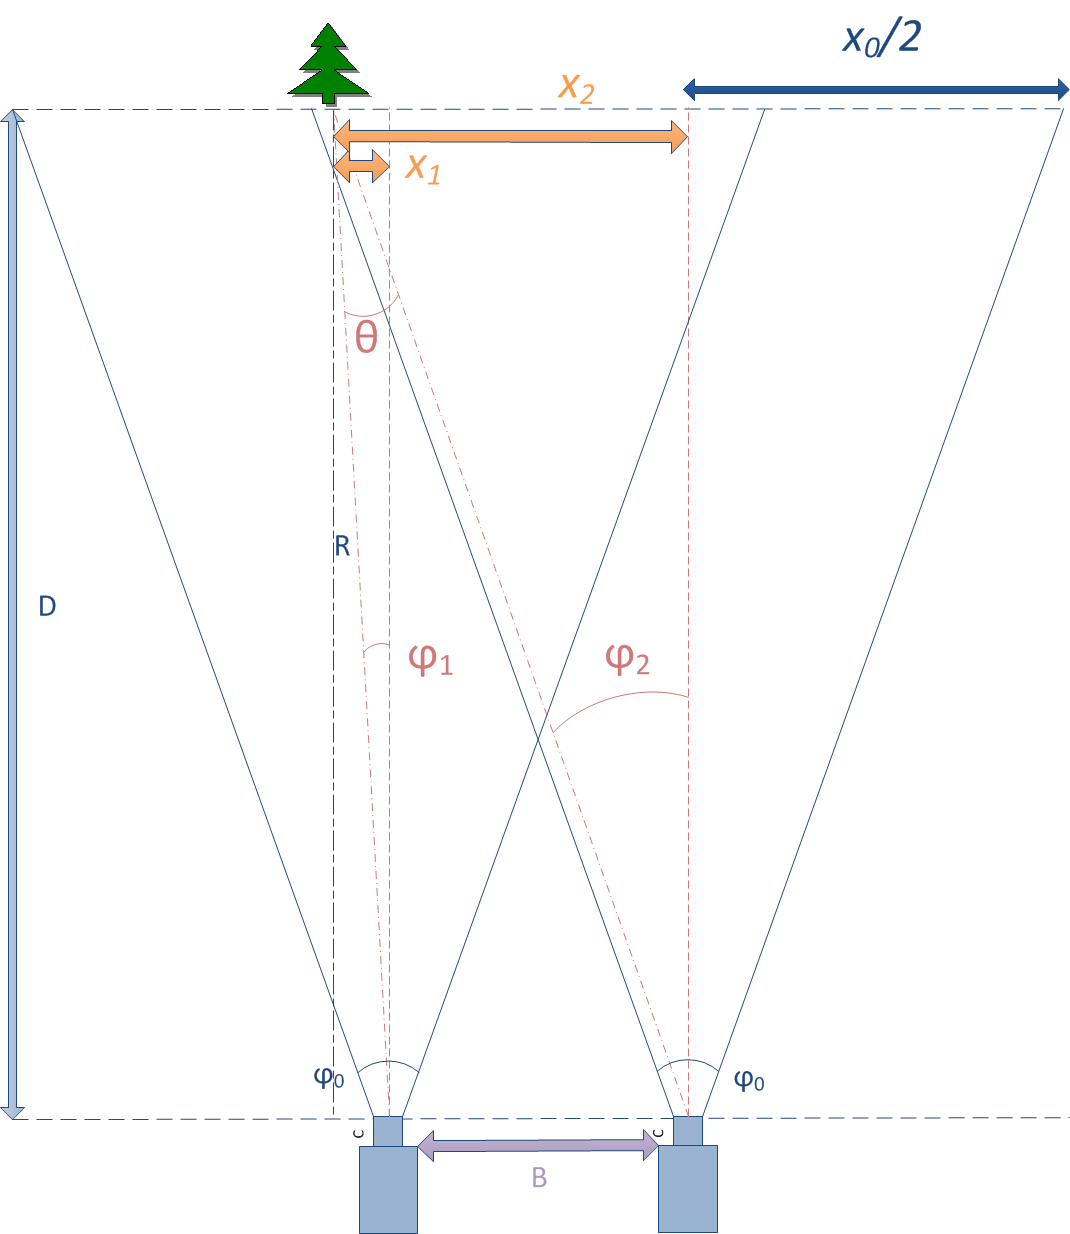
\includegraphics[width=\textwidth,height=\textheight,keepaspectratio]{Figures/problem2.png}
\caption{Problem 2 - Object is to the same side in both cameras}
\label{problem_toleft}
\end{figure}

\section{Object is in front of a camera}
The distance, $D$, in this problem is given by:

\begin{equation} \label{eq:p3:D}
D = B \tan\left(\frac{\pi}{2} - \varphi_{2}\right)
\end{equation}
Where $\varphi_2$ can be found from equation \ref{eq:p2:phi2}. 
\begin{figure}
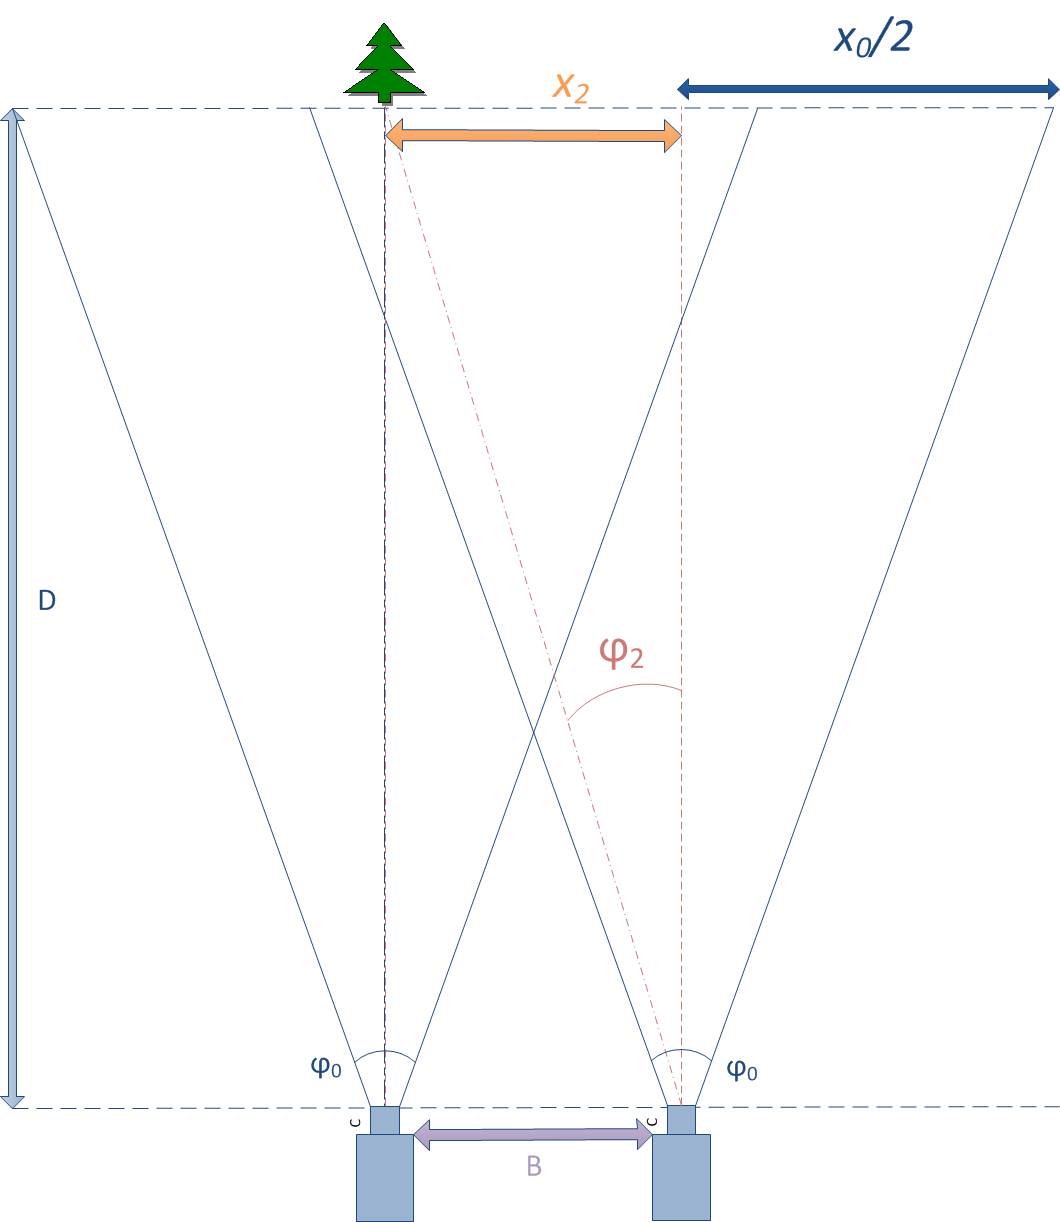
\includegraphics[width=\textwidth,height=\textheight,keepaspectratio]{Figures/problem3.png}
\caption{Problem 3 - Object is directly in front of a camera}
\label{fig:problem_infront}
\end{figure}